\section{Evaluation}
\label{Evaluation}

%\subsection{Einleitung}
%\label{Einleitung}
Die Evaluation soll kl"aren, wie genau die neuronalen Netze die Aufgaben der Klassifizierung und Generierung ausf"uhren k"onnen. Um eine m"oglichst gute L"osung zu bekommen wird in der Evaluation untersucht, welche Features und Parameter sich als vorteilhaft erweisen und wann Features und Verarbeitungsschritte "uberfl"ussig sind. $L$, $M$, $N$ und $H$ bezeichnen die in Kapitel~\ref{Klassifizierung} erl"auterten Features. $L$ ist die Lernrate, $M$ das Momentum, $N$ die Anzahl der Trainingsepochen und $H$ beschreibt die Anzahl der Knoten in der verdeckten Schicht. Hat ein Netz mehrere verdeckte Schichten, werden diese durch Kommata getrennt.

\subsection{Klassifizierung}
\label{EvalKlassifizierung}
Bei der Klassifizierung handelt es sich um eine Aufgabe bei der ein Lastgang in ein Zustandsprofil umgewandelt werden soll. Eingabe sind Merkmale des Lastgangs und Ausgabe ist eine Klassenzuordnung f"ur jeden Datenpunkt.\\
Als Ma{\ss} f"ur die G"ute der Klassifizierung dient die Genauigkeit und damit die Frage, bei wie vielen Datenpunkten (Instanzen) die richtige Klasse klassifiziert wurde. Eine Gewichtung der Fehlertypen findet zun"achst nicht statt.\\

Zu Beginn besch"aftigen wir uns mit der Auswahl des richtigen Zeitfensters. Es zeigt sich schnell, dass selbst dieser begrenzte Featureraum bereits mehrere lokale Optima aufweist, siehe dazu Tabelle~\ref{EvalZeit}. Die besten Ergebnisse liefert der Zeitraum von 3 Sekunden um den Zeitpunkt t, f"ur diesen werden weitere Tests durchgef"uhrt.\\

Zun"achst variieren wir die Epochen \textit{N}. Festzustellen ist, dass eine Erh"ohung der Epochen "uber 1000 keine Verbesserung der Genauigkeit mehr mit sich bringt. Die Normalisierung der Wirkleistung verschlechtert das Ergebnis. Dies ist vermutlich auf die vorherige Quantisierung der Daten zur"uckzuf"uhren, diese sorgt daf"ur, dass die Normalisierung die Werte eher streut statt gl"attet. \\
Das Hinzuf"ugen eines zweiten Hiddenlayer f"uhrt zu einer Verbesserung der Klassifikationsgenauigkeit. Die Ver"anderung von Lernrate und Momentum, beziehungsweise das Hinzuf"ugen eines dritten Hiddenlayer bringen jedoch keine weiteren Verbesserungen. Die Ergebnisse f"ur die Tests mit verschiedenen Parametern sind in Tabelle~\ref{EvalParam} zusammengefasst.\\

Die speziell f"ur die Waschmaschine gesuchten Features schneiden schlechter als die Zeitreihen ab (Tabelle~\ref{EvalExp}). Dies soll kein gro{\ss}er R"uckschlag f"ur diese Arbeit sein, die Zeitreihen sind leichter zu berechnen und besitzen allgemeineren Charakter. Letztere Eigenschaft scheint nicht nur praktisch, sondern auch der Klassifikation dienlich zu sein.\\

Ein genauerer Blick auf die Konfusionsmatrix~\ref{EvalConf} des Netzes mit dem besten Ergebnis verr"at, dass die meisten Verwechselungen zwischen Klasse 3, 4 und 5 auftreten. Das Netz hat hier offenbar Probleme die Unterschiede in den Verbrauchsspitzen zu erkennen. Diese Art von Fehlern umfasst 62 Instanzen und somit knapp $2/3$ der Fehlklassifikationen. \\
Die 22 Fehler bei denen ein \textit{Off-Zustand} als Klasse 1 klassifiziert wurden sind im Prinzip \textit{off-by-one-Fehler}. Das Netz erkennt nicht die semantische Bedeutung des Features t+0 und klassifiziert auch solche Zeitpunkte als \textit{On-Zustand}, bei denen die Werte t+1,2,3 bzw. t-1,2,3 gr"o{\ss}er Null sind, obwohl t+0 gleich Null ist. Die restlichen Fehlklassifikationen sind "ahnlich zu betrachten, insgesamt machen die \textit{off-by-one-Fehler} mit 33 Instanzen gut $1/3$ der Fehlklassifikationen aus. \\

\begin{table}[h]
\begin{tabular}{l|p{4cm}|p{4cm}|l}
Features & Korrekt klassifizierte Instanzen & Inkorrekt klassifizierte Instanzen & Genauigkeit  \\
\hline
t-10 bis t+10 & 29263 & 740 & 97.5336\% \\
t-9 bis t+9 & 29551 & 452 & 98.4935\% \\
t-8 bis t+8 & 29652 & 351 & 98.8301\% \\
t-7 bis t+7 & 29612 & 391 & 98.6968\% \\
t-6 bis t+6 & 29372 & 631 & 97.8969\% \\
t-5 bis t+5 & 29249 & 754 & 97.4869\% \\
t-4 bis t+4 & 29802 & 201 & 99.3301\% \\
t-3 bis t+3 & 29876 & 127 & 99.5767\% \\
t-2 bis t+2 & 29093 & 910 & 96.967\% \\
t-1 bis t+1 & 26526 & 3477 & 88.4112\% \\
t+0 & 29508 & 495 & 98.3502\% 
\end{tabular}
\caption[Genauigkeit der Zeitreihen Features]{Genauigkeit des Netzes bez"uglich verschiedener L"angen von Zeitreihen, Netz mit Weka Standardkonfiguration (-L 0.3 -M 0.2 -N 500 -H (\# Features+\# Klassen)/2)}
\label{EvalZeit}
\end{table}


\begin{table}[p]
\begin{tabular}{l|l|l|l|p{3cm}|p{3cm}|l}
L & M & N & H & Korrekt klassifizierte Instanzen & Inkorrekt klassifizierte Instanzen & Genauigkeit  \\
\hline
0.3 & 0.2 & 500 & 5 & 29535 & 486 & 98.3811\% \\
0.3 & 0.2 & 1000 & 5 & 29853 & 168 & 99.4404\% \\
0.3 & 0.2 & 1500 & 5 & 29535 & 486 & 98.3811\% \\
\end{tabular}
\caption[Spezielle Features]{Genauigkeit des Netzes bez"uglich verschiedener Parameter des Netzes, es werden die speziellen Features verwendet}
\label{EvalExp}
\end{table}

\begin{table}[p]
\begin{tabular}{l|l|l|l|p{1.5cm}|p{3cm}|p{3cm}|l}
L & M & N & H & Normali-siert & Korrekt klassifizierte Instanzen & Inkorrekt klassifizierte Instanzen & Genauigkeit  \\
\hline
0.3 & 0.2 & 500 & 6 & nein & 29876 & 127 & 99.5767\% \\
0.3 & 0.2 & 500 & 6 & ja & 29870 & 133 & 99.5567\% \\
0.3 & 0.2 & 1000 & 6 & nein & 29888 & 115 & 99.6167\% \\
0.3 & 0.2 & 1000 & 6 & ja & 29882 & 121 & 99.5967\% \\
0.3 & 0.2 & 1500 & 6 & nein & 29883 & 120 & 99.6\% \\
0.3 & 0.2 & 1500 & 6 & ja & 29870 & 133 & 99.5567\% \\
\hline
0.3 & 0.2 & 1000 & 13,6 & nein & 29908 & 95 & 99.6834\% \\
0.2 & 0.2 & 1000 & 13,6 & nein & 29755 & 248 & 99.1734\% \\
0.4 & 0.2 & 1000 & 13,6 & nein & 29543 & 460 & 98.4668\% \\
0.3 & 0.1 & 1000 & 13,6 & nein & 29886 & 117 & 99.61\% \\
0.3 & 0.3 & 1000 & 13,6 & nein & 29540 & 463 & 98.4568\% \\
0.3 & 0.2 & 1000 & 7,13,6 & nein & 28368 & 1635 & 94.5505\%
\end{tabular}
\caption[Parameterver"anderungen beste Zeitreihe]{Genauigkeit des Netzes bez"uglich verschiedener Parameter des Netzes, als Zeitreihe wird der Zeitraum t-3 bis t+3 verwendet, zus"atzlich wird gegen die normalisierte Wirkleistung getestet}
\label{EvalParam}
\end{table}


\begin{table}[p]
\begin{tabular}{llllll|l}
a & b & c & d & e & f & $\leftarrow$ classified as  \\
\hline
3670 & 22 & 0 & 0 & 0 & 0 & a = 0  \\
0 & 20984 & 0 & 0 & 0 & 2 & b = 1  \\
0 & 2 & 4762 & 0 & 0 & 0 & c = 2  \\
0 & 3 & 0 & 39 & 15 & 0 & d = 3  \\
0 & 2 & 0 & 18 & 52 & 12 & e = 4  \\
0 & 2 & 0 & 0 & 17 & 401 & f = 5  \\
\end{tabular}
\caption[Konfusionsmatrix]{Konfusionsmatrix des Netzes mit den Features t-3 bis t+3 und den Parametern -L 0.3 -M 0.2 -N 1000 -H 13,6}
\label{EvalConf}
\end{table}

\newpage
\subsection{Generierung}
\label{EvalGenerierung}
Die Aufgabe der Generierung erstellt aus einem Zustandsprofil wieder einen Lastgang, dazu darf die Klasse des zu prognostizierenden Datenpunktes und die ihm vorhergegangenen Datenpunkte verwendet werden. Als Anfangswert kann man Werte des \textit{Off-Zustands} annehmen und dann iterativ neue Datenpunkte berechnen beziehungsweise prognostizieren. F"ur die Evaluation werden die vorhergegangenen Datenpunkte als gegeben betrachtet. \\

Zu Beginn steht auch hier wieder die Auswahl des richtigen Zeitfensters. Tabelle~\ref{GenZeit} zeigt die Ergebnisse bez"uglich der Standardkonfiguration von Weka, die Verwendung der letzten 7 Sekunden stellt das Optimum im Suchbereich dar, f"ur dieses werden weitere Tests durchgef"uhrt.\\

Bei der Variierung der Parameter wird mit der Anzahl der Epochen und der Breite des Hiddenlayers begonnen. Es zeigt sich, dass ein schmaler Hiddenlayer besser die Charakteristik des Lastgangs erkennen kann, als ein breiter. Beim anschlie{\ss}enden variieren von Lernrate und Momentum zeigt sich au{\ss}erdem, dass f"ur beide Parameter niedrige Werte das Ergebnis verbessern, dies gilt insbesondere f"ur die Kombination von niedriger Lernrate mit niedrigem Momentum. Die Ergebinsse finden Sie in Tablle~\ref{GenParam}. 
Danach werden noch einmal die Epochen erh"oht um festzustellen, ob sich dadurch das Ergebnis noch weiter verbessern l"asst, dies ist jedoch schon nach 2000 Epochen nicht mehr der Fall. \\

Abbildung~\ref{GenWasch} zeigt in blau einen echten Waschgang und in gr"un einen, mit der Kenntnis vergangener Werte, Vorhergesagten. Gut zu erkennen ist die Tendenz des Netzes den Lastgang zu gl"atten, Spitzen und Schluchten im Verbrauch weichen im prognostizierten Verlauf weniger stark vom Mittelwert der Klasse ab.

\begin{table}[h]
\begin{tabular}{l|p{4cm}|p{4cm}}
Features & Root Mean Squared Error & Root Relative Squared Error \\
\hline
t-10 bis t-1 & 87.7099 & 12.8235\% \\
t-9 bis t-1 & 91.2275 & 13.3378\% \\
t-8 bis t-1 & 91.0262 & 13.3084\% \\
t-7 bis t-1 & 84.3952 & 12.3389\% \\
t-6 bis t-1 & 99.7641 & 14.5859\% \\
t-5 bis t-1 & 94.7697 & 13.8557\% \\
t-4 bis t-1 & 93.1525 & 13.6193\% \\
t-3 bis t-1 & 84.6953 & 12.3828\% \\
t-2 bis t-1 & 94.5766 & 13.8275\% \\
t-1 & 91.6551 & 13.4004\% 
\end{tabular}
\caption[Generierung mit Zeitreihen Features]{Genauigkeit der Generierung bez"uglich verschiedener L"angen von Zeitreihen, die Klasse des zu klassifizierenden Datenpunktes ist ebenfalls gegeben. Netz mit Weka Standardkonfiguration (-L 0.3 -M 0.2 -N 500 -H (\# Features+\# Klassen)/2)}
\label{GenZeit}
\end{table}

\begin{table}[h]
\begin{tabular}{l|l|l|l|p{3cm}|p{3cm}}
L & M & N & H & Root Mean Squared Error & Root Relative Squared Error \\
\hline
0.3 & 0.2 & 500 & 7 & 84.3952 & 12.3389\% \\
0.3 & 0.2 & 500 & 14 & 88.0205 & 12.869\% \\
0.3 & 0.2 & 1000 & 7 & 81.7189 & 11.9476\% \\
0.3 & 0.2 & 1000 & 14 & 88.9724 & 13.0081\% \\
0.3 & 0.2 & 1500 & 7 & 81.0541 & 11.8504\% \\
0.3 & 0.3 & 1500 & 7 & 83.2135 & 12.1662\% \\
0.3 & 0.1 & 1500 & 7 & 79.5297 & 11.6276\% \\
0.1 & 0.2 & 1500 & 7 & 72.1011 & 10.5415\% \\
0.1 & 0.1 & 1500 & 7 & 71.9262 & 10.5159\% \\
0.05 & 0.1 & 1500 & 7 & 68.3153 & 9.988\% \\
0.01 & 0.1 & 1500 & 7 & 66.8258 & 9.7702\% \\
0.005 & 0.1 & 1500 & 7 & 66.6262 & 9.741\% \\
0.3 & 0.2 & 2000 & 7 & 81.096  & 11.6639\% \\
0.1 & 0.2 & 2000 & 7 & 72.1756 & 10.5524\% \\
0.01 & 0.1 & 2000 & 7 & 66.9218 & 9.7843\% \\
0.01 & 0.1 & 2500 & 7 & 67.0246 & 9.7993\% \\
0.01 & 0.1 & 3000 & 7 & 67.113 & 9.8122\% \\
0.01 & 0.1 & 3000 & 14 & 66.8768 & 9.7777\% \\
0.01 & 0.1 & 4000 & 14 & 66.9756 & 9.7921\% \\


\end{tabular}
\caption[Parameterver"anderungen f"ur Generierung]{Genauigkeit der Generierung bez"uglich verschiedener Parameter des Netzes, als Zeitreihe wird der Zeitraum t-7 bis t-1 und die Klasse des Datenpunktes verwendet}
\label{GenParam}
\end{table}

\begin{figure}[ht]
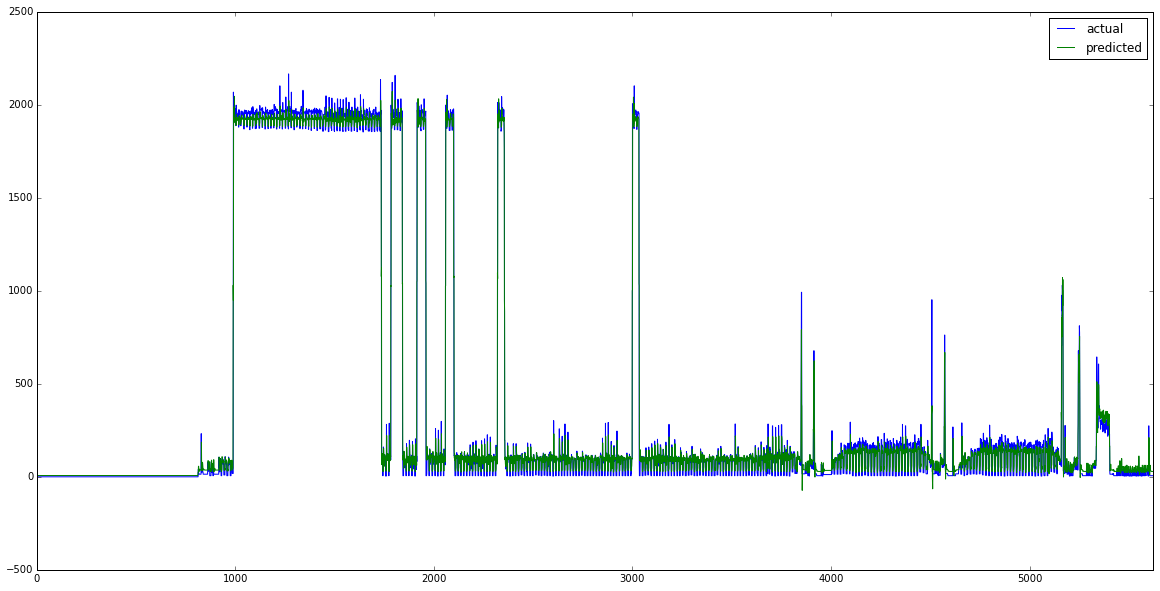
\includegraphics[height=0.7\textwidth , angle=90]{1_Grafiken/predicted.png}
	\caption[Typischer Waschgang, vorhergesagt]{Ein typischer Waschgang, blau zeigt den tats"achlichen Lastgang, gr"un den von Netz vorhergesagten. Als Grundlage f"ur die Vorhersage dienen die Werte t-7 bis t-1 und die Klasse von t+0, das Netz wurde mit den Parametern -L 0.01 -M 0.1 -N 4000 -H 14 erstellt}
\label{GenWasch}
\end{figure}